\documentclass[tikz,border=8pt]{standalone}
\usepackage[T1]{fontenc}
\usepackage{helvet}
\renewcommand{\familydefault}{\sfdefault}
\usetikzlibrary{positioning,arrows.meta,fit,backgrounds}
\definecolor{c1}{HTML}{1F4E79}\definecolor{f1}{HTML}{DCE9F5}
\definecolor{c2}{HTML}{7F4F00}\definecolor{f2}{HTML}{FBEBD0}
\definecolor{c3}{HTML}{2E6B30}\definecolor{f3}{HTML}{DDF0DD}
\definecolor{c4}{HTML}{5B2C83}\definecolor{f4}{HTML}{EBDDF5}
\definecolor{gr}{HTML}{555555}
\begin{document}
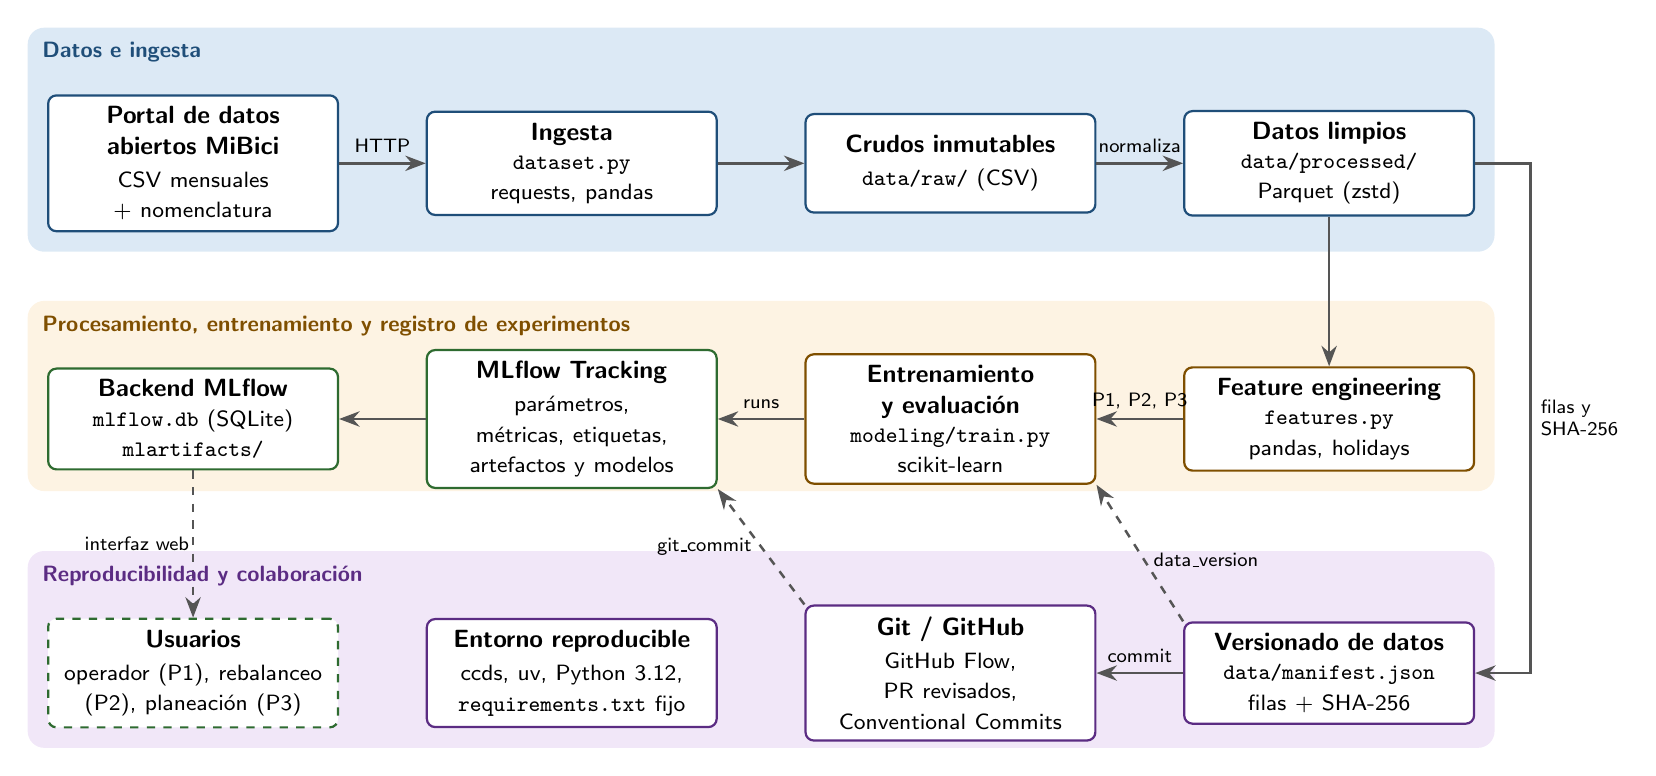
\begin{tikzpicture}[
  font=\small,
  box/.style={draw=#1, fill=white, rounded corners=3pt, line width=0.8pt, align=center,
              minimum height=1.25cm, text width=3.4cm, inner sep=4pt, execute at begin node={\hyphenpenalty=10000\exhyphenpenalty=10000}},
  arr/.style={-{Stealth[length=2.6mm]}, line width=0.9pt, draw=gr},
  lane/.style={fill=#1, rounded corners=6pt, inner sep=7pt},
  lab/.style={font=\bfseries\footnotesize, anchor=north west}
]
% Fila 1: datos
\node[box=c1] (portal) {\textbf{Portal de datos abiertos MiBici}\\[1pt]\footnotesize CSV mensuales + nomenclatura};
\node[box=c1, right=1.1cm of portal] (ingesta) {\textbf{Ingesta}\\[1pt]\footnotesize \texttt{dataset.py}\\ requests, pandas};
\node[box=c1, right=1.1cm of ingesta] (raw) {\textbf{Crudos inmutables}\\[1pt]\footnotesize \texttt{data/raw/} (CSV)};
\node[box=c1, right=1.1cm of raw] (proc) {\textbf{Datos limpios}\\[1pt]\footnotesize \texttt{data/processed/}\\ Parquet (zstd)};
% Fila 2: procesamiento y entrenamiento
\node[box=c2, below=1.9cm of proc] (feat) {\textbf{Feature engineering}\\[1pt]\footnotesize \texttt{features.py}\\ pandas, holidays};
\node[box=c2, left=1.1cm of feat] (train) {\textbf{Entrenamiento y evaluación}\\[1pt]\footnotesize \texttt{modeling/train.py}\\ scikit-learn};
\node[box=c3, left=1.1cm of train] (mlflow) {\textbf{MLflow Tracking}\\[1pt]\footnotesize parámetros, métricas, etiquetas, artefactos y modelos};
\node[box=c3, left=1.1cm of mlflow] (store) {\textbf{Backend MLflow}\\[1pt]\footnotesize \texttt{mlflow.db} (SQLite)\\ \texttt{mlartifacts/}};
% Fila 3: versionado y uso
\node[box=c4, below=1.9cm of feat] (manif) {\textbf{Versionado de datos}\\[1pt]\footnotesize \texttt{data/manifest.json}\\ filas + SHA-256};
\node[box=c4, left=1.1cm of manif] (git) {\textbf{Git / GitHub}\\[1pt]\footnotesize GitHub Flow, PR revisados, Conventional Commits};
\node[box=c4, left=1.1cm of git] (env) {\textbf{Entorno reproducible}\\[1pt]\footnotesize ccds, uv, Python 3.12, \texttt{requirements.txt} fijo};
\node[box=c3, left=1.1cm of env, dashed] (users) {\textbf{Usuarios}\\[1pt]\footnotesize operador (P1), rebalanceo (P2), planeación (P3)};

\draw[arr] (portal) -- node[above,font=\scriptsize]{HTTP} (ingesta);
\draw[arr] (ingesta) -- (raw);
\draw[arr] (raw) -- node[above,font=\scriptsize]{normaliza} (proc);
\draw[arr] (proc) -- (feat);
\draw[arr] (feat) -- node[above,font=\scriptsize]{P1, P2, P3} (train);
\draw[arr] (train) -- node[above,font=\scriptsize]{runs} (mlflow);
\draw[arr] (mlflow) -- (store);
\draw[arr] (proc.east) -- ++(0.7,0) |- node[pos=0.25,right,font=\scriptsize,align=left]{filas y\\SHA-256} (manif.east);
\draw[arr] (manif) -- node[above,font=\scriptsize]{commit} (git);
\draw[arr, dashed] (manif.north west) -- node[pos=0.45,right=2pt,font=\scriptsize,inner sep=1pt]{data\_version} (train.south east);
\draw[arr, dashed] (git.north west) -- node[pos=0.5,left=2pt,font=\scriptsize,inner sep=1pt]{git\_commit} (mlflow.south east);
\draw[arr, dashed] (store.south) -- node[pos=0.5,left,font=\scriptsize,inner sep=1pt]{interfaz web} (users.north);

\coordinate (t1) at ([yshift=6mm]portal.north);
\coordinate (t2) at ([yshift=6mm]store.north);
\coordinate (t3) at ([yshift=6mm]users.north);
\begin{scope}[on background layer]
  \node[lane=f1, fit=(portal)(proc)(t1)] (l1) {};
  \node[lane=f2!60, fit=(store)(feat)(t2)] (l2) {};
  \node[lane=f4!70, fit=(users)(manif)(t3)] (l3) {};
\end{scope}
\node[lab] at ([xshift=2pt,yshift=-2pt]l1.north west) {\color{c1}Datos e ingesta};
\node[lab] at ([xshift=2pt,yshift=-2pt]l2.north west) {\color{c2}Procesamiento, entrenamiento y registro de experimentos};
\node[lab] at ([xshift=2pt,yshift=-2pt]l3.north west) {\color{c4}Reproducibilidad y colaboración};
\end{tikzpicture}
\end{document}
